%%%%%%%%%%%%%%%%%%%% author.tex %%%%%%%%%%%%%%%%%%%%%%%%%%%%%%%%%%%
%
% sample root file for your "contribution" to a contributed volume
%
% Use this file as a template for your own input.
%
%%%%%%%%%%%%%%%% Springer %%%%%%%%%%%%%%%%%%%%%%%%%%%%%%%%%%


% RECOMMENDED %%%%%%%%%%%%%%%%%%%%%%%%%%%%%%%%%%%%%%%%%%%%%%%%%%%
\documentclass[graybox]{svmult}

% choose options for [] as required from the list
% in the Reference Guide

\usepackage{mathptmx}       % selects Times Roman as basic font
\usepackage{helvet}         % selects Helvetica as sans-serif font
\usepackage{courier}        % selects Courier as typewriter font
\usepackage{type1cm}        % activate if the above 3 fonts are
                            % not available on your system
%
\usepackage{makeidx}         % allows index generation
\usepackage{graphicx}        % standard LaTeX graphics tool
                             % when including figure files
\usepackage{multicol}        % used for the two-column index
\usepackage[bottom]{footmisc}% places footnotes at page bottom

\usepackage{multirow}
\usepackage{listings}


% see the list of further useful packages
% in the Reference Guide

\makeindex             % used for the subject index
                       % please use the style svind.ist with
                       % your makeindex program

%%%%%%%%%%%%%%%%%%%%%%%%%%%%%%%%%%%%%%%%%%%%%%%%%%%%%%%%%%%%%%%%%%%%%%%%%%%%%%%%%%%%%%%%%

\begin{document}

\title*{Fuzzy Simulation of Human Behaviour in the Health-e-Living System}
% Use \titlerunning{Short Title} for an abbreviated version of
% your contribution title if the original one is too long
%\author{Name of First Author and Name of Second Author}
\author{Remberto Martinez \and Marcos Tong \and Luis Diago \and Timo Nummenmaa \and Jyrki Nummenmaa}
\authorrunning{Martinez et. al} 
% Use \authorrunning{Short Title} for an abbreviated version of
% your contribution title if the original one is too long
%\institute{Name of First Author \at Name, Address of Institute, \email{name@email.address}
%\and Name of Second Author \at Name, Address of Institute \email{name@email.address}}
\institute{
Remberto Martinez \at ExtensiveLife Oy, Lohkaretie 2 B 9, 33470 Tampere, Finland, \email{remberto@health-e-living.com}
\and
Marcos Tong \at ExtensiveLife Oy, Lohkaretie 2 B 9, 33470 Tampere, Finland, \email{marcos@health-e-living.com}
\and
Luis Diago \at Interlocus Inc, Yokohama City 226-8510 and Meiji Institute for Advanced Study of Mathematical Sciences Meiji University, 4-21-1 Nakano, Tokyo 164-8525, Japan , \email{ldiago@i-locus.com}
\and 
Timo Nummenmaa \at University of Tampere, Finland, \email{timo.nummenmaa@staff.uta.fi}
\and 
Jyrki Nummenmaa \at University of Tampere, Finland, \email{jyrki.nummenmaa@staff.uta.fi}
}

%
% Use the package "url.sty" to avoid
% problems with special characters
% used in your e-mail or web address
%
\maketitle

\abstract*{This chapter shows an application of fuzzy set theory to preventive health support systems where adherence to medical treatment is an important measure to promote health and reduce health care costs. Preventive health care information technology systems design include ensuring adherence to treatment through Just-In-Time Adaptive Interventions (JITAI). Determining the timing of the intervention and the appropriate intervention strategy are two of the main difficulties facing current systems. In this work, a JITAI system called Health-e-living (Heli) was developed for a group of patients with type-2 diabetes. During the development stages of Heli it was verified that the state of each user is fuzzy and it is difficult to get the right moment to send motivational message without being annoying. A fuzzy formula is proposed to measure the adherence of patients to their goals. 
As the adherence measurement needed more data, it was introduce the DisCo software toolset for formal specifications, the modelling of human behaviour and health action process approach (HAPA) to simulate the interactions between users of the Heli system. The effectiveness of interventions is essential in any JITAI system and the proposed formula allows Heli to send motivational messages in correspondence with the status of each user as to evaluate the efficiency of any intervention strategy.}

\abstract{This chapter shows an application of fuzzy set theory to preventive health support systems where adherence to medical treatment is an important measure to promote health and reduce health care costs. Preventive health care information technology systems design include ensuring adherence to treatment through Just-In-Time Adaptive Interventions (JITAI). Determining the timing of the intervention and the appropriate intervention strategy are two of the main difficulties facing current systems. In this work, a JITAI system called Health-e-living (Heli) was developed for a group of patients with type-2 diabetes. During the development stages of Heli it was verified that the state of each user is fuzzy and it is difficult to get the right moment to send motivational message without being annoying. A fuzzy formula is proposed to measure the adherence of patients to their goals. 
As the adherence measurement needed more data, it was introduce the DisCo software toolset for formal specifications, the modelling of human behaviour and health action process approach (HAPA) to simulate the interactions between users of the Heli system. The effectiveness of interventions is essential in any JITAI system and the proposed formula allows Heli to send motivational messages in correspondence with the status of each user as to evaluate the efficiency of any intervention strategy.}


\section{Introduction}



Developing better systems to capture and track patient-specific receipt of preventive health services delivered anywhere and over time will be critical to optimising performance measurement and reducing unnecessary duplication of care\cite{Bowen2017}. In theory, Just-in-Time Adaptive Interventions (JiTAIs)\cite{Nahum-Shani} are a persuasive technology which promise to empower personal behavioural goals by optimising treatments to situational context and user behaviours~\cite{Murray2016}.JiTAI design aim is to provide the right type/amount of support, at the right time, by adapting to an individual's changing internal and contextual state\cite{Nahum-Shani}. However, People's health determinants are difficult to model because of their inherent uncertainty, the complex interactions among them, as well as the considerable number of variables and lack of precise mathematical models\cite{Hekler2016}. 

Fuzzy set theory provides the necessary tools when someone intends to work with vague, ambiguous, imprecise, noisy or missing information\cite{Gursel2016, Bingchuan2012, Giabbanelli2014, Giabbanelli2006}. In~\cite{Giabbanelli2006}, the authors present a general view of the current applications of fuzzy logic in medicine and bioinformatics. Several fuzzy-logic based context models~\cite{Bingchuan2012}, and a related context-aware reasoning middleware that provides a personalized, flexible and extensible reasoning framework have been developed to infer how personal behaviour is expected to change under a given intervention~\cite{Giabbanelli2014}. 


In our previous work  presented at ISFUROS 2017~\cite{rem2017} we have applied fuzzy modelling to calculate progress and send motivation emails to users depending on the type of adherence to the system (high, medium or low). The acquired data is related to nutrition, mood and physical activity mainly. However, the results were only preliminary because the sample size was not large and there were missing data. In this chapter we add the DisCo software toolset ~\cite{Disco} to simulate users missing data in order to validate our previous modelling by Fuzzy Rules extraction from Time Series and using rules to reproduce real models and extract new knowledge from the simulations. 
The data simulated includes the HAPA model ~\cite{MacPhail}, the adherence formula specifications developed in our previous work and the human behaviour model reported in~\cite{Brailsford2016}
to demonstrate the advantages of using fuzzy rules extracted from real system data, compare these rules validity in simulated data  and to discovers a new user behaviour or a new user type that is not available in the real system or in the scientific literature.

The rest of the chapter is organised as follows. First, section \ref{sec.heli} introduces the Heli system, our previous fuzzy formula for measuring user's adherence to de system and the modelling of Human Behaviour with a simplified HAPA model. Section \ref{sec.helimodel} briefly describes the Disco simulation and Heli adherence formula specification. Section \ref{sec.rules} presents the proposed method to extract rules from the simulations and section \ref{sec.results} compares the results of the proposed approach with the approach reported in~\cite{Brailsford2016} to demonstrate the advantages of modelling human behaviour during fuzzy adherence calculation. Finally, conclusions and future works are presented in section~\ref{sec.conclusions}.

\section{Health-e-living (Heli) System}
\label{sec.heli}

 Health-e-living (Heli)\cite{rem2012} is a mobile solution to deliver preventive, educational and promotional health to all citizens comfortable with IT technologies independently of their age or geographical location. Heli uses the metaphor of social networks to improve health habits of persons connected to their support network in real life (family, friends, and colleagues). Figure~\ref{Fig.heli} shows the logical solution provided by the Heli system.
 The EMA  (Ecological Momentary Assessment) data collected about user activities related to biometrics, mental, nutrition or physical activity are gathered and transmitted using a mobile device with communication capabilities. Users can annotate the data in history or discuss with experts or own support communities. The data is stored in a private cloud after user's consent and is used to generate automatic reports on goal progress and trends for both users and coaches. 
 The Heli system provides its users with periodical interactions, educational material and motivational messages to help them achieve their selected goals. At the same time provides tools to coaches for easier daily management, survey preparations and guidance material creation.
 
\begin{figure}
  \begin{center}
  \begin{tabular}{c}
    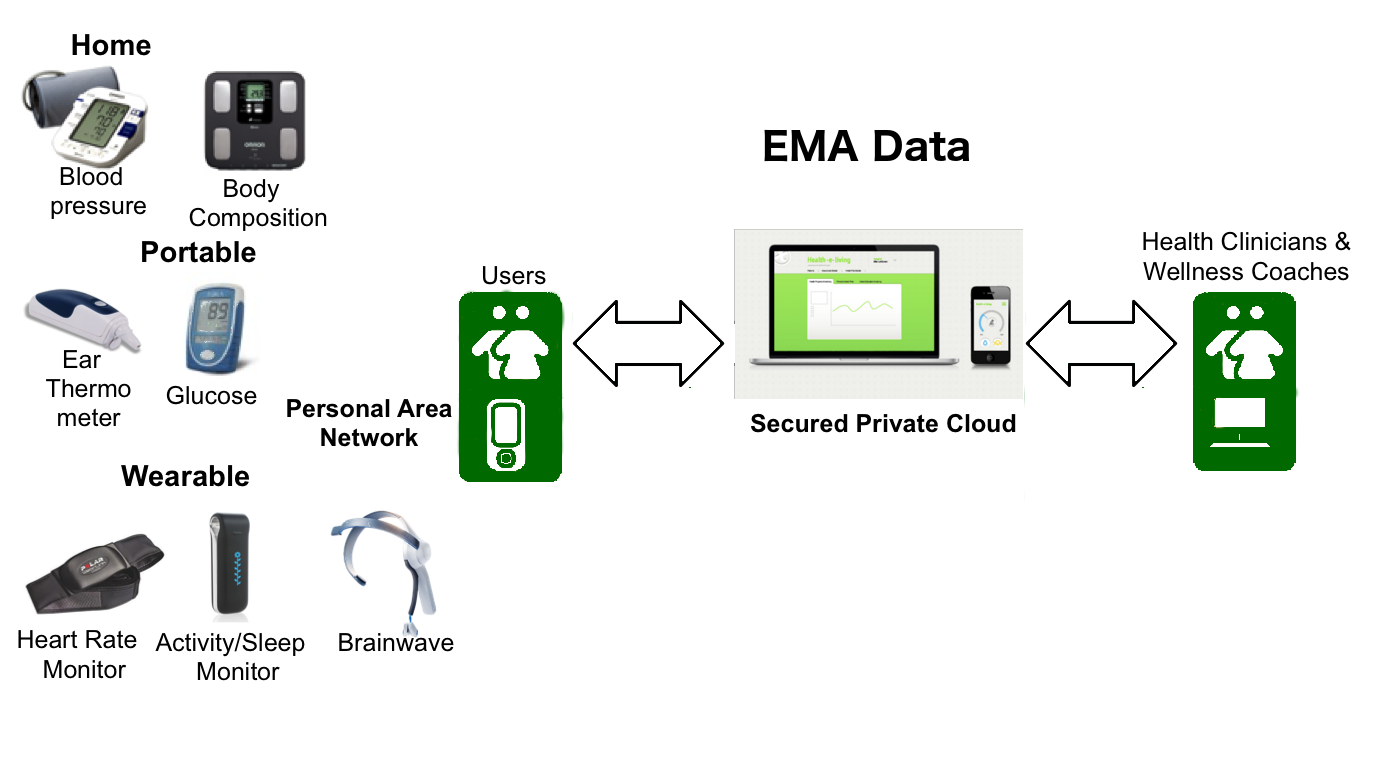
\includegraphics[scale=0.5]{LogicalSolutionNow.png}\\
    \end{tabular}
    \caption{Logical Solution provided by the Heli system\cite{rem2012}}
     \label{Fig.heli}
\end{center}
\end{figure} 

\subsection{Fuzzy  Adherence Measurement}

People's health determinants are difficult to model because of their inherent uncertainty, the complex interactions among them, as well as the considerable number of variables and lack of precise mathematical models. This was the main motivation to use a fuzzy approach as a  practical option to model the adherence to a treatment and healthy lifestsyle of a patient in the Heli system. In Heli, two variables are combined for the evaluation of patients' status: the progress of the proximal outcomes $\Delta x = \|x - g_i\|$  and the patient adherence to the system $y = F(x,z)$. Note that the value of $y$ depends on the inputs $x$ (i.e. proximal outcomes) which are controlled by the patients and the contextual inputs $z$ (e.g. environment) which are not controlled by the patients. Progress indicates how close a patient is to completing the outcomes $g_{i(1\leq i \leq n)}$ and the adherence measures how effective the system is in its intervention. The adherence is modelled as a fuzzy weighted average involving type-1 (T1) fuzzy sets as follows~\cite{Liu2008}:
\begin{equation}
y = \frac{\sum_{i=1}^n w_i x_i}{\sum_{i=i}^n w_i}
\label{Eq.AdheranceFWA}
\end{equation}
In (\ref{Eq.AdheranceFWA}), $w_i$ are weights that act upon proximal outcomes $x_i$. While it is always true that the sum of the normalized weights that act upon each $x_i$ add to one, it is not a requirement that the sum of the unnormalized weights must add to one. The adherence is calculated as an average of several goals, and gives an idea of how well the system goes with the goals of the patients. Every goal $g_i$ is defined on an interval $g_i \in [g_{-}, g^{+}]$ and the values of $y_{-}$ and $y^{+}$ are computed accordingly as follows:
\begin{equation}
 	y_{-}(x)= \left\{ 
	\begin{array}{lcr}
        1,	         & if &(x \geq g_{-})\\
        x/g_{-} 	 & if &(0<x<g_{-})\\
        1                & &otherwise
	\end{array}
	\right \},
 	y^{+}(x)= \left\{ 
	\begin{array}{lcr}
        1,	         & if &(x \leq g^{+}),\\
        \frac{2g^{+}- x}{g^{+} }	 & if &(g^{+}<x<2g^{+} )\\
        0                & if & x \geq 2g^{+}\\
        1                & & otherwise
	\end{array}
	\right \}.
\label{Eq.Adherance}
\end{equation}
An example of positive goal to achieve would be to increase fruits consumption as a minimum of 5 fruit portions in a week or to walk a minimum of 10000 steps a day. For this type of goals  $g_{-}$ it is enough to achieve the minimum in order to have 100 \% of completion. Similarly for negative goal, and example could be to decrease sugary beverage consumption with a maximum of 1 glass of soda in a week.  This type of goal $g^{+}$ would achieve 100  \% of completion with no data entry or zero amount of beverage portions consumed.

As it was mentioned before, the choice of the time interval between decision points can have a dramatic impact on the ability of a user to achieve its goals. Patient progress is calculated daily and adherence is added to the system weekly but it is calculated every two weeks because we can not calculate without data. The time interval between decision points is set to two-weeks to see how many entries there are in that period. As long as adhesion is closer to 1 the system is more effective.

\subsection{Modelling Human Behaviour with a simplified HAPA model}

HAPA is designed as a sequence of two continuous self-regulatory processes, a goal-setting phase (motivation) and a goal-pursuit phase (volition). The second phase is subdivided into a pre-action phase(volition) and an action phase(maintenance) (see~Fig.\ref{Fig.hapa})

\begin{figure}
  \begin{center}
  \begin{tabular}{c}
    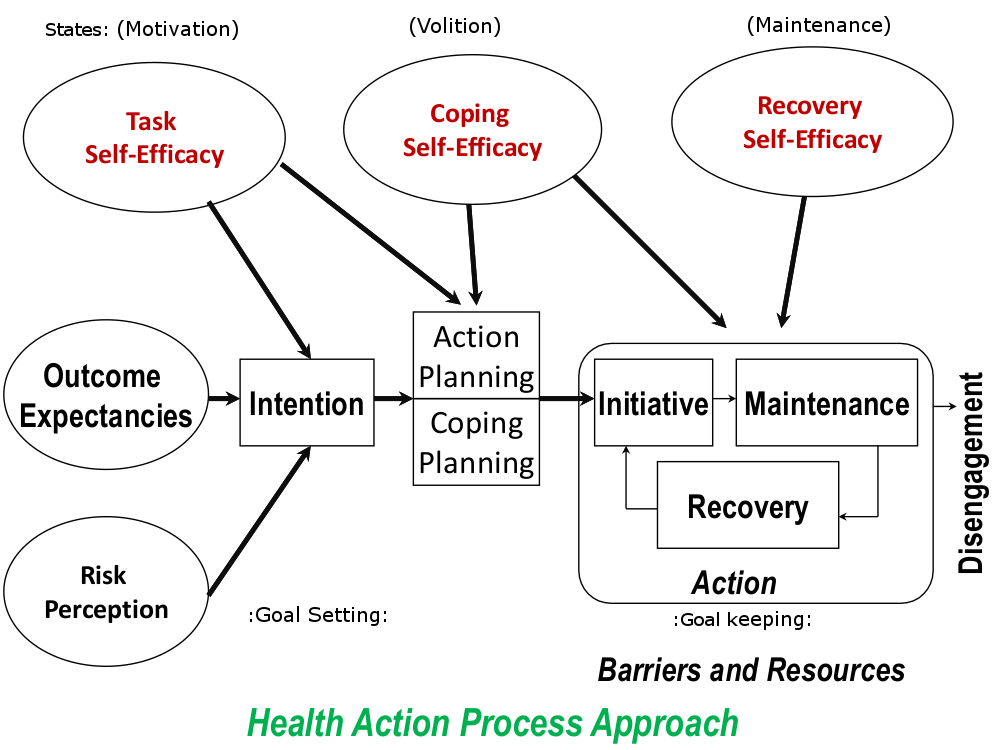
\includegraphics[scale=0.4]{hapa_firem.png}\\
    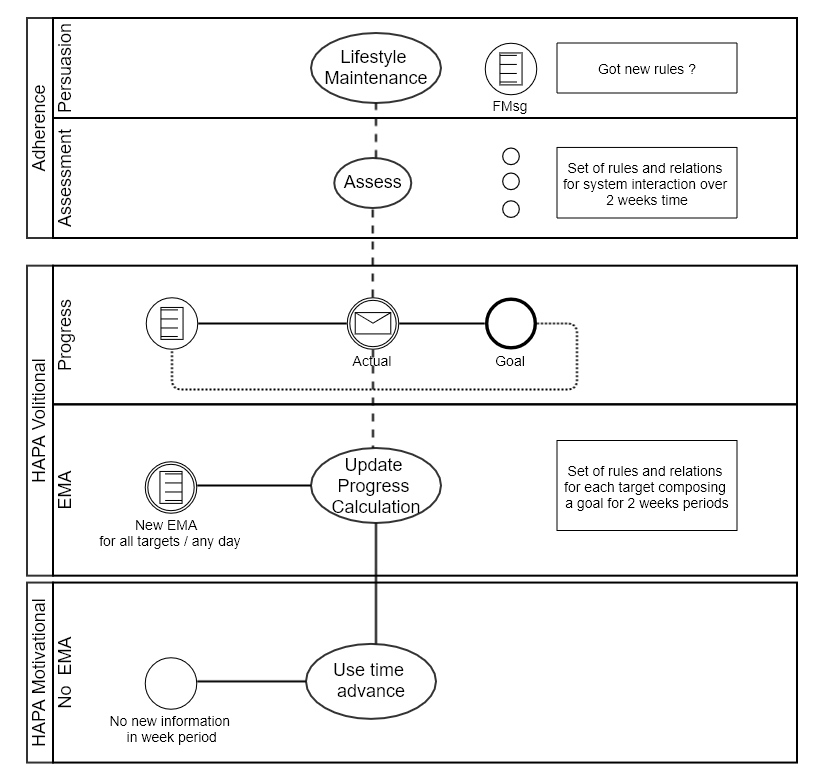
\includegraphics[scale=0.4]{Hapa.png}\\
    \end{tabular}
    \caption{Health Action Process Approach \cite{rem2012}}
     \label{Fig.hapa}
\end{center}
\end{figure} 

In this work we use the stage model; the stage approach assumes that change is non-linear and consists of several qualitative steps that reflect different mindsets of people.
We could model the efficacy of HeLi as the probability of compliance with Health Goal set at the evaluation time ( 2 weeks ) or just simply the probability of an intended Health Behaviour Change Compliance.

\begin{equation}
 	HBCC(t) =  CH(t) * MA(t) * P(t)
\label{Eq.HBChange}
\end{equation}

Where CH(t) is adherence history over the time the system is used and n is the number of previous inputs
\begin{equation}
           CH(t) =   1 - (0.1)^ {n(t)} 
\label{Eq.ComplianceHistory}
\end{equation}
 MA(t) is the Motivation to comply with Health Goal selected according to your personal motivation (Mi) and believes (Bi) at any time,
 \begin{equation}
           MA(t) =  \sum_{i=1}^n M_i * B_i 
\label{Eq.MotivationHistory}
\end{equation}
  P(t) is the Perceived Self-Efficacy over time, including outcomes expectations (Ok) and risk perception (Rk)  during intention formation.
  \begin{equation}
           P(t) =  \sum_{k=1}^n O_k * R_k
\label{Eq.PerceivedSE}
\end{equation}

    Brailsford used a probability to participate in treatment of 0.85 \cite{Brailsford2016} for patients diagnosed with cancer.  In Heli the real data is collected from patients diagnosed with Diabetes Type 2 risk and so the probability of any user to input data after selecting a personal goal over time is equivalent to the probability of a user participating to a Health Behaviour Change during the period of time when system is used. Heli system as a preventative health process tries to persuades users to change towards a healthy behaviour by assessing the data collected over the period of two weeks. For any lifestyle change to be consider as a sticky habit the period of assessment should be greater  than two weeks and so is the period used for evaluating the efficacy of the system. 
    
   Assuming that motivation to provide personal data is constant for all users, it is possible to model three main user types influenced by a goal self awareness and the normative believe of that entering data in the system will contribute to achieving the set goal as low ( 0.5), moderate high (0.8) and high (1.0) and that will lead to provide more entries during the time span of two weeks. It is possible to assume in a first modelling phase that P is always 1.
   
With this simplistic model, it is possible to generate simulation data so that is representative of the results obtained with real data. In this model the simulator could be configured to generate an input event based on certain probability. In this first iteration the user behaviour is able to form an intention, plan and take basic actions. The next step would be to model a user behaviour that is influenced by the environment and will change the perceived self-efficacy in time.

The main contribution of HAPA model is allowing perceived self-efficacy to change over time in situations where user needs to cope with setbacks or recover from life challenges. In this iteration is possible to add two more properties to the user model: emotional commitment ( 1, can cope or 0.1, not ) and failure learning ( 1, can recover or 0.2, not ). Now the simulated data allows a user to react on the event of receiving a motivational message or not. In this phase the value of P will be calculated over the assessment period of time.
Figure ~\ref{Fig.hapa} shows on top the basic HAPA model with its three user states: Motivation, Volition and Maintenance. On the bottom is represented how the model is used in system Heli where Volition and Maintenance are combined in one state as HAPA\_Volition.

\section {Heli Adherence specification for DisCo Simulation}
\label{sec.helimodel}

As the amount of real data available in the Heli system was limited and the amount of available data from real users was not substantial enough, in this chapter we describe Fuzzy Adherence Simulation using a HAPA model for User's behaviour in a DisCo formal specification environment as a method to generate more data resembling the data observed in the real system.

There were 126 users registered in Heli from 2013/07 to 2017/03 (including 8 system administrators, 20 coaches and 98 patients mainly related with type-2 diabetes ). Fig.~\ref{Fig.Weight-Goals} shows patients weight (44-125Kg ) and the distribution of the number of goals selected by the participants.
\vspace*{-\baselineskip}\begin{figure}[h]
  \begin{center}
  \begin{tabular}{c}
     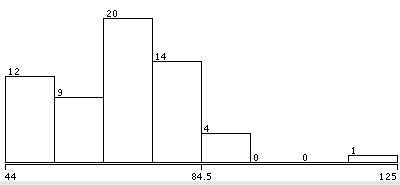
\includegraphics[width=0.8\textwidth]{Weight.png}\\
          a) Weight\\
   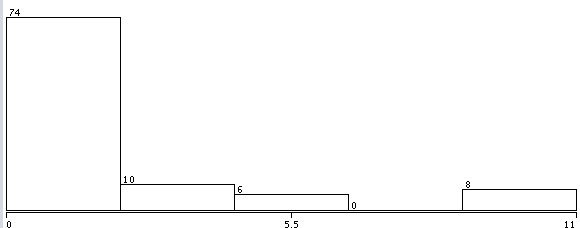
\includegraphics[width=0.8\textwidth]{Goals.png}\\
 b) Number of goals selected by participants\\
    \end{tabular}
    \caption{Statistics of the data collected for 98 patients registered in Heli from 2013/07 to 2017/03}
     \label{Fig.Weight-Goals}
\end{center}
\end{figure} 

\subsection {Computing Adherance and state of the patients}
\label{sec.patient_states}

Several authors~\cite{Murray2016, Nahum-Shani, MacPhail} have emphasized the importance of having computational models of human behaviour to monitor the dynamics of an individual's internal state and context in real time. The adaptation requires monitoring the individual to decide (a) whether the individual is in a state that requires support; (b) what type (or amount) of support is needed given the individual's state; and (c) whether providing this support has the potential to disrupt the desired process. In our previous work we focus on the design and evaluation of effective interventions exploring patients self-reporting states and sending motivational messages based on a dimensional approach. Table~\ref{Tab.States} shows 7 dimensions, 13 states and some examples of motivational messages used in the intervention. Note that the messages are associated to the dimensions and not to the states of the patients, since the states vary over time and in some cases the states were not reported during the system test stage (e.g. states marked with "-" in the table). Current probabilities of the states are included within parenthesis. Motivational messages are sent to the patients based on the computed adherence to their proximal outcomes and their reported states (i.e. feedbacks). 

\begin{table}[h]
\caption{ Health-e-Living Intervention Approach}
\begin{tabular}{ | l | c | l |}
\hline
Dimension & Patient States & Examples of motivational messages\\ \hline
\multirow{5}{*}{1. Physiological} &  & Think of the week. What has caused your  \\
 & sick/ill  (0.0285)  & physiological response? What could you change  \\
 & stressed (0.1285)  & in your behaviour to next time avoid these \\ 
&    tired (0.3857)  & (e.g. go to bed earlier, eat more regularly, \\ 
&   & eating proper meals etc.)  \\ \hline
\multirow{3}{*}{2. Optimism} & energetic (0.0285) & Sometimes things that are out of our control  \\
 &   confident  (0.0714)  & prevent us from fulfilling our\\
 &  content (-) &  good intentions. Try again next week!\\ \hline
\multirow{3}{*}{3. Time } &  & You can learn from every experience. \\ 
&  busy (0.2142)   &What will you do similarly/differently\\
&  &  next time? \\ \hline
\multirow{3}{*}{4. Drive} &  & It?s hard work to change an old habit, \\
& hungry/thirsty (-) & and in the long term a warm and caring \\
& &  attitude helps more than criticism\\ \hline
\multirow{2}{*}{5. Social } &  socially pressured (0.0428) & Think of the situation at hand. Does it  \\
 &  unsupported (-) & matter that you deviated from your plan? \\ \hline
\multirow{2}{*}{6. Emotional } & happy (0.0857)  & Keep going and see how the changes \\ 
& & affect your well-being!\\ \hline
\multirow{2}{*}{7. Discourage } &  disappointed(0.0142) & What has helped you succeed before? \\
 &  unmotivated(-)  & Could you apply those skills to this situation?\\ \hline
\hline
\end{tabular}
\label{Tab.States}
\end{table}

The Waikato Environment for Knowledge Analysis (WEKA)~\cite{WEKA} software was used to predict the state of one patient (id=19). The patient provided 46 feedbacks to de system including 8 states: tired (14), stressed (5), busy(14), sick/ill(2), energetic(1), confident(3), socially pressured(3) and happy(4). The number in parenthesis represents the times the state was provided. NaiveBayes, MLPClassifier, AdaBoostM1 and RBFNetwork classifiers were tested with one feature computed by (\ref{Eq.AdheranceFWA}) and the 8 states provided by the patient. Using a 10-fold cross-validation method the accuracy of the classifiers was 23.9130\%,  26.0870\%, 32.6087\% and 34.7826\% respectively. The accuracy of the classifiers is still very low due to class overlapping (e.g. tired, stressed, busy and socially pressured are very similar) and missing values in the computation of the fuzzy adherence for the patients. In Heli, the number of users with fuzzy adherence was very small (25/98 $\approx$ 25.5\%) because most users (73/98 $\approx$ 74.5\%) prefer to use the system to store daily data without a specific goal. As the emotional dimensions used in the research may not be the most adequate, later on we use machine learning tools to enhance the effectiveness of Heli based on computational models of human behaviour like the health action process approach (HAPA)\cite{MacPhail}.

\subsection {Disco Simulation}

A formal specification should state precisely what a completed piece of software is supposed to do, but not how the task should be achieved \cite{Diller}. Formal specifications are a powerful method for modelling system behaviour, usually used in software development. DisCo is primarily intended for the specification of reactive systems and its semantics have been defined with the Temporal Logic of Actions \cite{Lamport}. The DisCo software toolset \cite{Aaltonen}, originally developed at the Tampere University of Technology, includes a compiler for compiling specifications created in the DisCo language, a graphical animation tool for animation and simulation of those specifications, and a scenario tool for representing execution traces as Message Sequence Charts. The human interaction with Heli system was specified using DisCo language and the simulation was executed in DisCo Animator version DisCo2000\^{}2  presented in \cite{Nummenmaa}.  

The main purpose of using DisCo specifications was to generate large amount of data as close as possible to the real world data collected while modelling a Human Behaviour that includes goals settings and the intention of acting upon the achievement of those goals. Running the simulation on DisCo animator supported the probability of a user providing input to the system, the adherence formula computation based on those entries and the probability of a user reacting after receiving a feedback message from Heli~\cite{rem2017}.
 
\begin{figure}
  \begin{center}
  \begin{tabular}{c}
    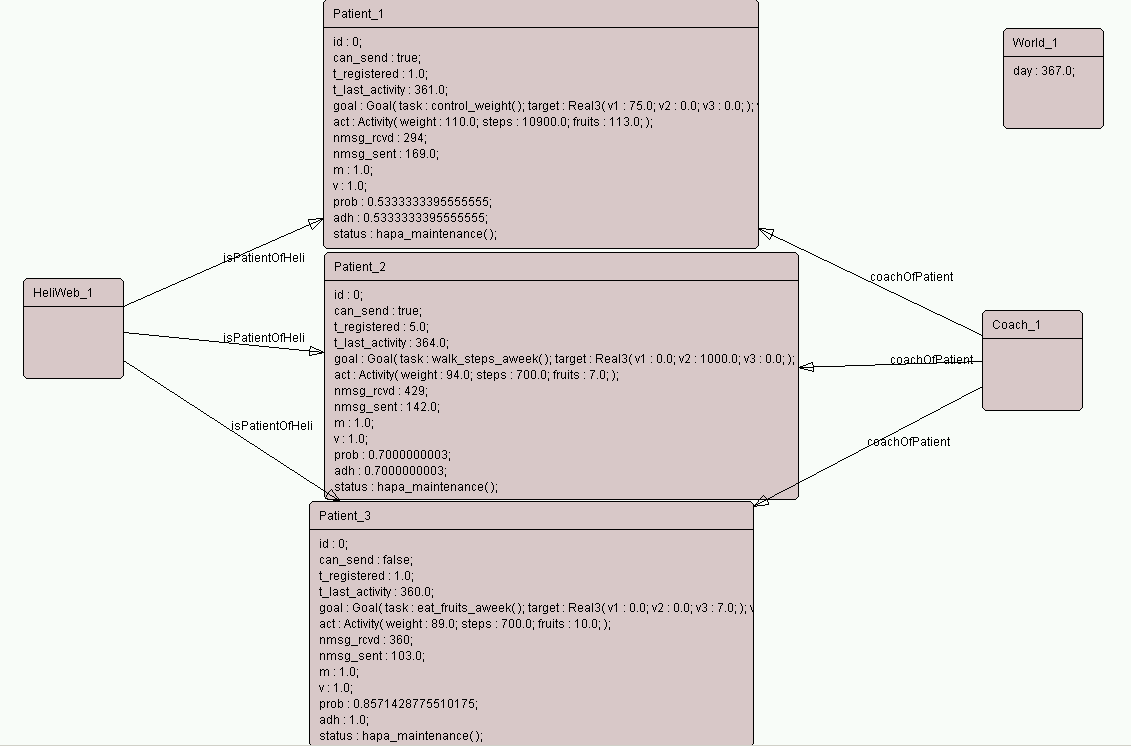
\includegraphics[scale=0.3]{DisCoAnimator.png}\\
    \end{tabular}
    \caption{DisCo Animator simulation in Heli world}
     \label{Fig.Animator}
\end{center}
\end{figure} 

In figure~\ref{Fig.Animator} the Heli simulation world consists of  four classes (patient, coach, Heli system and external world) that  can interact between each others through actions. Actions are enabled on the simulation according to their guard (simulation system state and relationship between classes). Enabled actions are selected  for execution nondeterministically (with weighted probability) in any specific execution time. When a participant user (patient) registers to Heli system and selects a goal (i.e monitor own weight),  a relation $isPatientOfHeli$ becomes active and indicates that the participant is already in the HAPA\_Motivational state. After running a simulation for a period equivalent to 367 days, the adherence to the system is observed and computed as the number of data inputs during a week period of time.  All modelled users were registered and defined a goal (on targets related to weight management, better nutrition and increase physical activity level), when no EMA entries are available in an evaluation period of time the simulation assigns the user to HAPA\_Motivational state. Later on when EMA entries are available during the week, the user is considered in HAPA\_Volitional or HAPA\_Maintenance state and the contents of each entries can be used to compute the progress over time towards the selected goal (see Fig.\ref{Fig.hapa}).

There are more than 1200 records per patient on average in the simulation. On each recorded entry, the simulation computes the probability of entering next input, the compliance history and the new value of adherence. Over the elapsed time of every two weeks, in the simulated world,  is possible to assess the value of adherence and based on that the system sends personalised messages according to user attribute compliance: not\_very\_active, active and very\_active. Since the simulation purpose was to generate data and not to represent the messages personalisation, the model increased the probability of sending more user activity for those users where the value of adherence was closer to 1( max).  This feature represents a participant resilience to cope with external environment setbacks. Resilience can be simplified to include user's emotional commitment and the ability to learn from a failure and to keep own goal as a user being of two types: responsive and not\_responsive. A user being responsive will have a high correlation with user in HAPA\_Volitional or HAPA\_Maintenance states, having moderately high adherence or  high adherence.

\begin{lstlisting}[language=Python, caption=Functions used in the Disco specification of Adherence in equation (\ref{Eq.AdheranceFWA})]

  function weightProgress(p: Patient): real is
    return 1.0 - abs(p.goal.target.v1 - p.act.weight)
		                  /(p.goal.target.v1);
  end;
  function stepsProgress(p: Patient): real is
     return 1.0 - (p.goal.target.v2 - p.act.steps)
                          /(p.goal.target.v2);
  end;
  function fruitsProgress(p: Patient): real is
     return 1.0 - (p.goal.target.v3 - p.act.fruits)
                          /(p.goal.target.v3);
  end;
  function computeAdherance(w:World; p:Patient) : real is	 		 
      return ( p.goal.w.v1 * weightProgress(p)  + 
            p.goal.w.v2 *   stepsProgress(p)  +
            p.goal.w.v3 * fruitsProgress(p) )   
         / (p.goal.w.v1 + p.goal.w.v2 + p.goal.w.v3) ;
   end;                    
\end{lstlisting}


\section {Fuzzy Rules extraction from Time Series}
\label{sec.rules}

As in our previous research the The Waikato Environment for Knowledge Analysis (WEKA)~\cite{WEKA} software was used to predict the state of above three patients. Instead of using the state reported by the patients, we used the three states included in the HAPA model (motivational, volitional and maintenance) to find a correspondence between the HAPA states and previous states reported by the real participants.  Using a 10-fold cross-validation method to predict the HAPA states with J48 classifier the accuracy was  99.76\%, 98.63\% and 99.20\% for each patient respectively. As the states of the patients are fixed by the simulator in the HAPA model, we find a mapping between the values of adherence in the precedents of the rules and the values of adherence in the previous states reported by the patient in the real Heli-system. In the current simulation of the system from the specifications, the HAPA states only depend on the registration process and the number of messages sent to the Heli by the Participants. There is not specification detailed for the changes in the HAPA states after the Patient entered the maintenance state. The factors to modify the states are currently under investigation and modelling.

\section {Preliminary Results}
\label{sec.results}

As the results in our previous research were only preliminary due to the small size of the the sample, in this chapter our experiments are focused to review the conditions of the real patients who participated in the Heli system. Using the simulation we intend to mimic real conditions with better models and extract new knowledge from the Disco simulations.  While the generated data does not reflect the real data exactly, it can be used to quickly validate the assumptions in the participants goal achievement progress and its system adherence calculation and then compare the results of the proposed approach with the approach reported in~\cite{Brailsford2016}. Fig.\ref{Fig.REALvsSIM} shows the probability distribution function for the adherence experimental data and the values of adherence computed by both simulation models. The main difference between both simulation models is that proposed model includes motivational messages sent by the coaches to the patients based on the values of adherence while Brailsford model does not includes motivational messages. The graph were computed by using the Matlab $fitdist$ function that creates a probability distribution object by fitting the Epanechnikov kernel function to the data. The values of the bandwidth were 0.1029, 0.0497 and 0.0744 for the real, Braidford and proposed simulated data respectively. Both models used in simulation were simplified to not include users personal motivation to achieve the intended goal, however the inclusion of HAPA model in the proposed allowed to predict the user state based on the number of inputs over time. The proposed model matches the adherence value increase of participants after receiving motivational messages as it was observed in the real data ~\cite{rem2017}.  Any user instance was allowed to have several goals at the same time, however due to time limitations the executed simulation assumed only one type of goal at the time. 

As it is shown in Fig.\ref{Fig.REALvsSIM}, the values of adherence are higher for the proposed approach ($0.54\pm0.32$ vs $0.51\pm0.32$) and also the graph is closer to the experimental/real graph. Although we did not compare the two distributions directly, we can see in the figure that in the extremes (adherence close to zero and adherence close to one) the distributions are very similar (they differ only in a scale factor). However, when the adherence values are between 0.4 and 0.8 the distributions do not look alike. This can be said to be due to the lack of data acquired during the real experiments and / or because the simulation is still far from including the aspects of reality that govern those cases where adherence has average values. The probability with which a patient sends data after receiving a message from a Coach has not been modelled either. The variation of the motivation over time has not been included either (the value of m = 1 was fixed during the simulation).
\begin{figure}
  \begin{center}
  \begin{tabular}{c}
    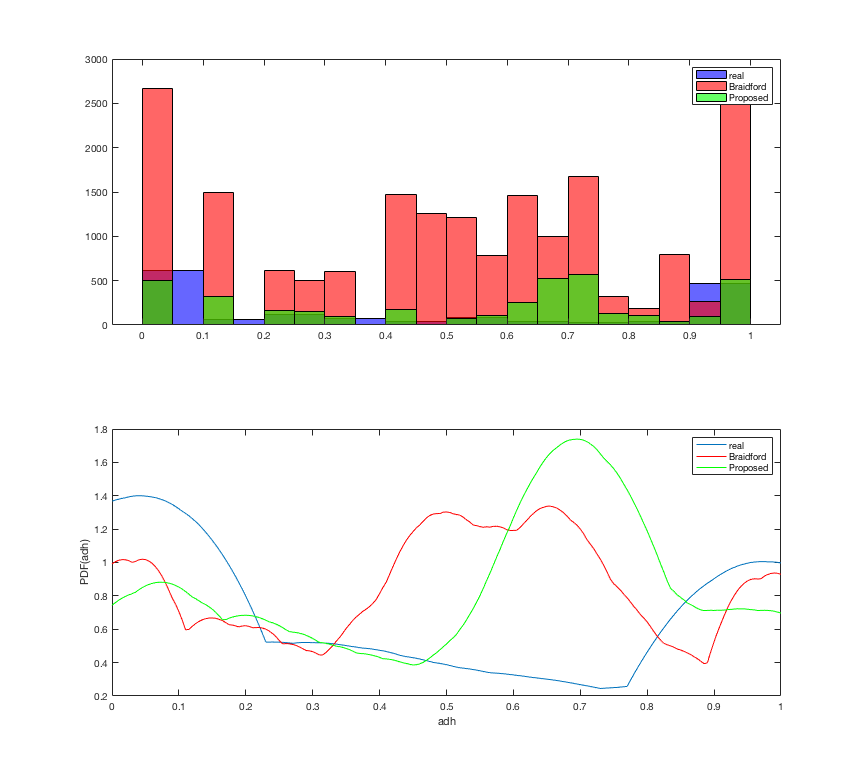
\includegraphics[scale=0.4]{REALvsBRAIDFORDvsPROPOSED.png}\\
    \end{tabular}
    \caption{Comparison of the histograms (upper part) and probability distribution function (PDF, lower part) for simulated and real values of adh.}
     \label{Fig.REALvsSIM}
\end{center}
\end{figure} 

The authors consider that the main objective of this work has been fulfilled, since we were able to increase the number of data by means of simulation and at the same time predict the states in which the patient is (according to HAPA) from the values of adherence computed by the proposed fuzzy formula in~(\ref{Eq.AdheranceFWA}). Finally, Figure~\ref{Fig.TimeSeries} shows the results of the simulations with Disco for 367 days with the 3 patients, the coach and the Heli system shown in Fig.\ref{Fig.Animator}. The average number of entries randomly generated was 2.4 times larger than the real data mainly because the number of real messages sent by the automatic Heli coach is smaller than those of the simulated. In the real Heli, the automatic coach generates a motivational message every 2 weeks for each patient, so it would be around 25 a year maximum or 50 if the patient provides more feedback (see the patient states in section \ref{sec.patient_states}). A human coach could generate a little bit more messages when supporting a real participant. In the simulation, the messages are generated daily in a random way so the number of records is larger. However, the simulation shows that some pattern of adherence exists according to the type of goal settled by the Patient. For example, Patient 1, that tried to control the weight below 75Kg never reached the goal during one year. On the contrary, Patient 2 and Patient 3 who settled their goals related with physical activities (e.g. walk more than 1000 steps a week) and nutrition (e.g. eat more than 7 fruits a week) could achieve their goal several times in the year.  As it is shown, Fig.~\ref{Fig.TimeSeries} shows a cyclic behaviour for Patient 2 and Patient 3. After the patient reached the goal the adherence is reduced. Although this behaviour was included in the simulated specification it can be consider in some agreement with real life. 
\begin{figure}
  \begin{center}
  \begin{tabular}{c}
    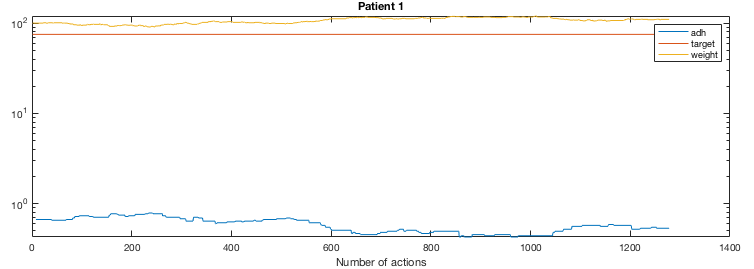
\includegraphics[scale=0.5]{Patient1-365-fuzzy.png}\\
    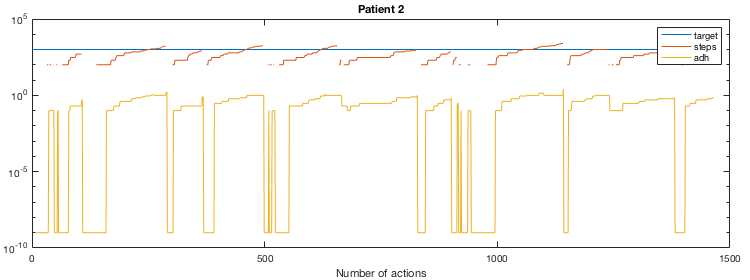
\includegraphics[scale=0.5]{Patient2-365-fuzzy.png}\\
    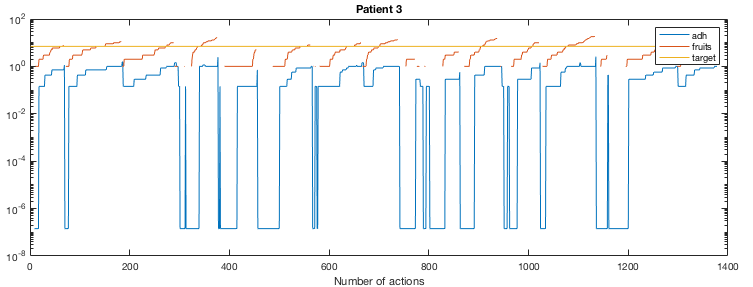
\includegraphics[scale=0.5]{Patient3-365-fuzzy.png}\\
    \end{tabular}
    \caption{Results of the simulations with Disco for 367 days with the 3 patients}
     \label{Fig.TimeSeries}
\end{center}
\end{figure} 

\section {Conclusions and Future Work}
\label{sec.conclusions}

JITAI systems like Heli appear to be a promising framework for developing mHealth interventions. In Heli, the number of users with fuzzy adherence was very small (25/98 $\approx$ 25.5\%) because most users (73/98 $\approx$ 74.5\%) prefer to use the system to store daily data without a specific goal. However, the  proposed interventions showed that even after several stress inputs patients do not leave the system. Although this research is still in its infancy, fuzzy measures like the proposed adherence formula constitute a practical option  to measure the way a patient approaches by successive approximations in time to a certain goal. The chapter showed by mean of simulation that there is a close correspondence between real world adherence of the patients and its computational model. 

The simplified model used in simulation did not include the reactiveness of users when receiving motivational messages from Heli automatic coach. The ways to adjust the number of registered records during simulation to agree with those of the real life is currently under investigation. Future works should expand the model to improve user personal motivation and perceived self-efficacy. For example by using the data available after user profiling or the data collected from system usage.  Another interesting approach would be to measure adherence when the model allows to change a goal after several weeks of simulation execution.

The introduction of  HAPA and human behaviour factors in the model required a better understanding of the user. The data collected from the real system was used to decide what relations and actions were the most important for state transitions and adherence computation.

While DisCo specifications were enough to describe the real system implementation, it could be expanded to give more freedom in modelling. The relationships between classes were enough to represent the Heli world in the simulator. Main limitations of current DisCo specification toolset is the ability to specify complex mathematical formulas and the reduced semantics set during the simulation preparation. The Animator tool was pleasant to use, however some improvements are needed to implement  external factors variability for the system under modelling during execution time. For the logs output processing it is desirable to add an export functionality to common standard formats like csv or database connectors. After several iterations of modelling, It was possible to generate large amount of data to discover new knowledge about real system. The data generated is found useful for other phases of software testing cycle in stage level systems. 

More research is required to understand the impact of behavioural interventions on real life user lifestyle achievements and what aspects of user motivation is triggering the intention of resilience improvements.

 
\begin{thebibliography}{99}

\bibitem{Aaltonen} T. Aaltonen, M. Katara, and R. Pitkanen. DisCo toolset - the new generation. Journal of Universal Computer Science, 7(1):3-18, 2001.

\bibitem{Bingchuan2012} Bingchuan Yuan, John Herbert, Fuzzy CARA - A Fuzzy-Based Context Reasoning System For Pervasive Healthcare,  Procedia Computer Science 10 (2012) 357 ? 365

\bibitem{Bowen2017} Michael E. Bowen, Deepa Bhat, Jason Fish, Brett Moran, Temple Howell-Stampley, Lynne Kirk, Stephen D. Persell, Ethan A. Halm, Improving Performance on Preventive Health Quality Measures Using Clinical Decision Support to Capture Care Done Elsewhere and Patient Exceptions.

\bibitem{Brailsford2016} Brailsford S.C. Healthcare: Human Behavior in Simulation Models. In: Kunc M., Malpass J., White L. (eds) Behavioral Operational Research 2016. Palgrave Macmillan, London.

\bibitem{Diller}  A. Diller. Z: An Introduction to Formal Methods. John Wiley \& Sons, Inc., 1990.

\bibitem{Disco} The DisCo project WWW page. At URL http://disco.cs.tut.fi on the World Wide Web. ( Accessed 16.4.2018)

\bibitem{Giabbanelli2006} Angela Torres and Juan J. Nieto Fuzzy Logic in Medicine and Bioinformatics, Journal of Biomedicine and Biotechnology Volume 2006, Article ID 91908, Pages 1?7, DOI 10.1155/JBB/2006/91908

\bibitem{Giabbanelli2014} Philippe J Giabbanelli and Rik Crutzen, Creating groups with similar expected behavioural response in randomized controlled trials: a fuzzy cognitive map approach, BMC Medical Research Methodology 2014, 14:130.

\bibitem{Gursel2016} Gursel G. Healthcare, uncertainty, and fuzzy logic. Digit Med 2016;2:101-12

\bibitem{Hafezi} Hooman Hafezi, Timothy L. Robertson, Greg D. Moon, Kit-Yee Au-Yeung, Mark J. Zdeblick, and George M. Savage, An Ingestible Sensor for Measuring Medication Adherence. IEEE Trans ON Biomedical Engineering, Vol. 62, No. 1, JANUARY 2015, pp 99-109

\bibitem{Hall2015} Amanda M. Hall, Steven J. Kamper, Marian Hernon, MPH,a Katie Hughes,  Chris Lonsdale, Deirdre A. Hurley and Raymond Ostelo, Measurement Tools for Adherence to Non-Pharmacologic Self-Management Treatment for Chronic Musculoskeletal Conditions: A Systematic Review, Arch Phys Med Rehabil. 2015 Mar;96(3):552-62. doi: 10.1016/j.apmr.2014.07.405.

\bibitem{Hekler2016} Hekler EB, Michie S, Pavel M, Rivera DE, Collins LM, Jimison HB, Garnett C, Parral S, Spruijt-Metz D.: Advancing Models and Theories for Digital Behavior Change Interventions, Am J Prev Med. 2016 Nov;51(5):825-832. doi: 10.1016/j.amepre.2016.06.013.

\bibitem{Lamport} L. Lamport. The temporal logic of actions. ACM Trans. Program. Lang. Syst., 16(3):872?923, 1994.

\bibitem{Liu2008} Feilong Liu,  and Jerry M. Mendel, Aggregation Using the Fuzzy Weighted Average as Computed by the Karnik-Mendel Algorithms, IEEE Trans. on Fuzzy Systems, Vol. 16, No. 1, pp-1 - 12 

\bibitem{MacPhail} Mariana MacPhail, Barbara Mullan, Louise Sharpe Carolyn MacCann and Jemma Todd Using the health action process approach to predict and improve health outcomes in individuals with type 2 diabetes mellitus. Diabetes, Metabolic Syndrome and Obesity: Targets and Therapy 2014:7 469?479.

\bibitem{Murray2016} Tylar Murray, Eric Hekler, Donna Spruijt-Metz, Daniel E. Rivera1, and Andrew Raij.: Formalization of Computational Human Behavior Models for Contextual Persuasive Technology, PERSUASIVE 2016, LNCS 9638, pp. 150?161, 2016. DOI: 10.1007/978-3-319-31510-2 13

\bibitem{Nahum-Shani} Inbal Nahum-Shani, \& Shawna N. Smith,  \& Bonnie J. Spring,  \&Linda M. Collins,  \& Katie Witkiewitz,  \& Ambuj Tewari, \& Susan A. Murphy, Just-in-Time Adaptive Interventions (JITAIs) in Mobile Health: Key Components and Design Principles for Ongoing Health Behavior Support, Annals of Behavioral Medicine 2016, doi: 10.1007/s12160-016-9830-8

\bibitem{Nguyen} Thi-My-Uyen Nguyen, Adam La Caze \& Neil Cottrell, What are validated self-report adherence scales really measuring?: a systematic review. British Journal of Clinical Pharmacology, 77:3 / 427?445

\bibitem{Nummenmaa} T. Nummenmaa. Executable Formal Specifications in Game Development: Design, Validation and Evolution. PhD  thesis, Tampere: Tampere University  Press 2013.

\bibitem{Prado} Carlos A Prado-Aguilar, Yolanda V Martinez, Yolanda Segovia-Bernal, Rosendo Reyes-Martnez and Raul Arias-Ulloa Performance of two questionnaires to measure treatment adherence in patients with Type-2 Diabetes, BMC Public Health. 2009 Jan 26;9:38. doi: 10.1186/1471-2458-9-38.

\bibitem{rem2012} Remberto Martinez and Marcos Tong: Can Mobile Health Deliver Participatory Medicine to  All Citizens in Modern Society? 4th International Conference on Well-Being in the Information Society, WIS 2012, Turku, 22 August 2012 - 24 August 2012 Pages 83-90.

\bibitem{rem2017}  Remberto Martinez, Marcos Tong and Luis Diago: Fuzzy Adherence Formula for the Evaluation of Just-In-Time Adaptive Interventions in the Health-e-living System. Proceedings of ISFUROS Symposium,  2017.

\bibitem{Wan} Wai Yin Lam and Paula Fresco.: Medication Adherence Measures: An Overview. BioMed Research International Volume 2015, Article ID 217047, 12 pages doi: 10.1155/2015/217047

\bibitem{WEKA} M. Hall, E. Frank, G. Holmes, B. Pfahringer, P. Reutemann, I.H. Witten, The WEKA Data Mining Software:  An Update, SIGKDD Explor Newsl. 11 (2009) 10?18. doi:10.1145/1656274.1656278.

\end{thebibliography}


\end{document}
